\documentclass[a4j]{jarticle}
%%  packages
\usepackage{amsmath,amssymb,ascmac}
\usepackage{bm}
\usepackage[dvipdfmx]{graphicx}
\usepackage{listings}
\usepackage[english]{babel}
\lstset{
 	%枠外に行った時の自動改行
 	breaklines = true,
 	%標準の書体
        basicstyle=\ttfamily\footnotesize,
        commentstyle=\footnotesize\bfseries,
        keywordstyle=\footnotesize\bfseries,
 	%枠 "t"は上に線を記載, "T"は上に二重線を記載
	%他オプション:leftline,topline,bottomline,lines,single,shadowbox
 	frame = single,
 	%frameまでの間隔(行番号とプログラムの間)
 	framesep = 5pt,
 	%行番号の位置
 	numbers = left,
	%行番号の間隔
 	stepnumber = 1,
	%タブの大きさ
 	tabsize = 4,
 	%キャプションの場所("tb"ならば上下両方に記載)
 	captionpos = t
}

%% math commands
\let \ds \displaystyle
\newcommand{\idiff}[3]{
  \frac{d^{#1} #2}{d #3^{#1}}
}
\newcommand{\diff}[3]{
  \frac{\mathrm{d}^{#1} #2}{\mathrm{d} #3^{#1}}
}
\newcommand{\pdiff}[3]{
  \frac{\partial^{#1} #2}{\partial #3^{#1}}
}



%% title configuration
\title{東京大学大学院情報理工学系研究科2016年度過去問}
\author{}
\date{}


%% headings
\pagestyle{headings}
\markright{東京大学大学院情報理工学系研究科2016年度過去問}




\begin{document}
%%  begin title page
\thispagestyle{empty}
\maketitle
\pagebreak


\section{}

\begin{screen}
 非負整数$n$について,トリボナッチ数列$\{T_n\}$は次のように定義される.
 
 $\ds \begin{cases} T_0 = T_1 = 0 \\ T_2 = 1 \\ T_{n+3} = T_{n+2} + T_{n+1} + T_{n} \quad(n \geq 0).\end{cases}$

 以下の設問に答えよ.
\end{screen}

\begin{screen}
 (1) 任意の非負整数 $n$ について式$(1.1)$を満たす行列$A$を求めよ.
 \begin{align*}
  \left(\begin{array}{l}T_{n+3} \\ T_{n+2} \\T_{n+1}\end{array}\right)
  =A\left(\begin{array}{l}T_{n+2} \\ T_{n+1} \\T_{n}\end{array}\right)\tag{1.1}
 \end{align*}
\end{screen}

$$A=\begin{pmatrix}
     1 & 1 & 1 \\
     1 & 0 & 0 \\
     0 & 1 & 0      
    \end{pmatrix}$$

\begin{screen}
 (2) 行列 $A$ のランクおよび特性方程式(固有値が満たす方程式)を求めよ.
\end{screen}

$A$の各列をなすベクトルは一次独立なので$A$のランクは$3$.

特性方程式は,

$$\left|\lambda I - A\right| = \lambda^3 - \lambda^2 - \lambda - 1 = 0$$

\begin{screen}
 (3) 行列 $A$ の固有値を $\lambda_1,\lambda_2,\lambda_3$とするとき,それぞれの固有値に対応する固有ベクトルを $\lambda_1,\lambda_2,\lambda_3$を用いて表せ.
\end{screen}

$\ds A \begin{pmatrix} x\\ y \\ z\end{pmatrix} = \lambda_i\begin{pmatrix} x\\ y \\ z\end{pmatrix}$
$\ds \Leftrightarrow
\left\{
\begin{array}[tb]{rrrrrr}
 x&+&y&+&z&=\lambda_i x \\
 x& & & & &=\lambda_i y \\
  & &y& & &=\lambda_i z \\
\end{array}
\right.
\Leftrightarrow
\begin{cases}
 (\lambda_i^3 - \lambda_i^2 - \lambda_i - 1)z &= 0 \\
 x &= \lambda_i^2 z \\
 y &= \lambda_i   z
\end{cases}
$

よって,固有値$\lambda_i$に対応する固有ベクトルは $\begin{pmatrix} \lambda_i^2\\ \lambda_i \\ 1\end{pmatrix}$
\begin{screen}
 (4) 行列 $A$ は実数固有値を一つのみ有することを示せ.また,これを $\lambda_1$ としたとき,$1<\lambda_1<2$であることを示せ.
\end{screen}

$f(\lambda)=\lambda^3-\lambda^2-\lambda-1$ と定義する.$f'(\lambda)=3\lambda^2-2\lambda-1>0$より$f(\lambda)$は狭義単調増加し,$f(1)=-2,$ $f(2)=1$より$f(\lambda)=0$の実数解は$1<\lambda<2$の範囲に1つのみとなる.これが$\lambda_1$に対応するので,実数固有値は1つのみで$1<\lambda_1<2$である.

\begin{screen}
 (5) ある複素定数$c_1,c_2,c_3$を用いて $T_n = c_1\lambda_1^n+c_2\lambda_2^n+c_3\lambda_3^n$と表せることを示せ.$c_1,c_2,c_3$の値を明示的に求める必要はない.
\end{screen}

正則行列$P$を用いて,$\ds A = P \begin{pmatrix} \lambda_1 & & \\ & \lambda_2 & \\ & & \lambda_3 \end{pmatrix} P^{-1}$と分解すると,

$$\begin{pmatrix} T_{n+2} \\ T_{n+1} \\ T_{n} \end{pmatrix} = A^n \begin{pmatrix} T_2 \\ T_1 \\ T_0 \end{pmatrix} = P \begin{pmatrix} \lambda_1^n & & \\ & \lambda_2^n & \\ & & \lambda_3^n \end{pmatrix}P^{-1}\begin{pmatrix} 1 \\ 0 \\ 0 \end{pmatrix}$$
と書けるので,$T_n$は$\lambda_1^n,\lambda_2^n,\lambda_3^n$の線型結合で表せる.

\begin{screen}
 (6) $\ds \lim_{n \rightarrow \infty} \frac{T_{n+1}}{T_n} = \lambda_1$ を示せ.
\end{screen}

解と係数の関係から$\lambda_1\lambda_2\lambda_3=1$,および$\lambda_3=\overline{\lambda}_2$より(4)の結果を用いて,$|\lambda_2|=|\lambda_3|<1<|\lambda_1|$が成り立つ.

$$\therefore \lim_{n \rightarrow \infty}\frac{T_{n+1}}{T_n}=\lim_{n \rightarrow \infty}\frac{c_1\lambda_1+c_2\lambda_2\left(\ds\frac{\lambda_2}{\lambda_1}\right)^n+c_3\lambda_3\left(\ds\frac{\lambda_3}{\lambda_1}\right)^n}{c_1+c_2\left(\ds\frac{\lambda_2}{\lambda_1}\right)^n+c_3\left(\ds\frac{\lambda_3}{\lambda_1}\right)^n}=\frac{c_1\lambda_1}{c_1}=\lambda_1$$

\section{}

\begin{screen}
 $xy$ 平面上の点$A(-1,2)$と点$B(1,2)$を結ぶ二回微分可能関数$y(x)$を考える.次に,曲線$y(x)$を$x$軸のまわりに回転させてできる筒状図形の外側の表面積を$S$とする.以下の設問に答えよ.
 
 \centering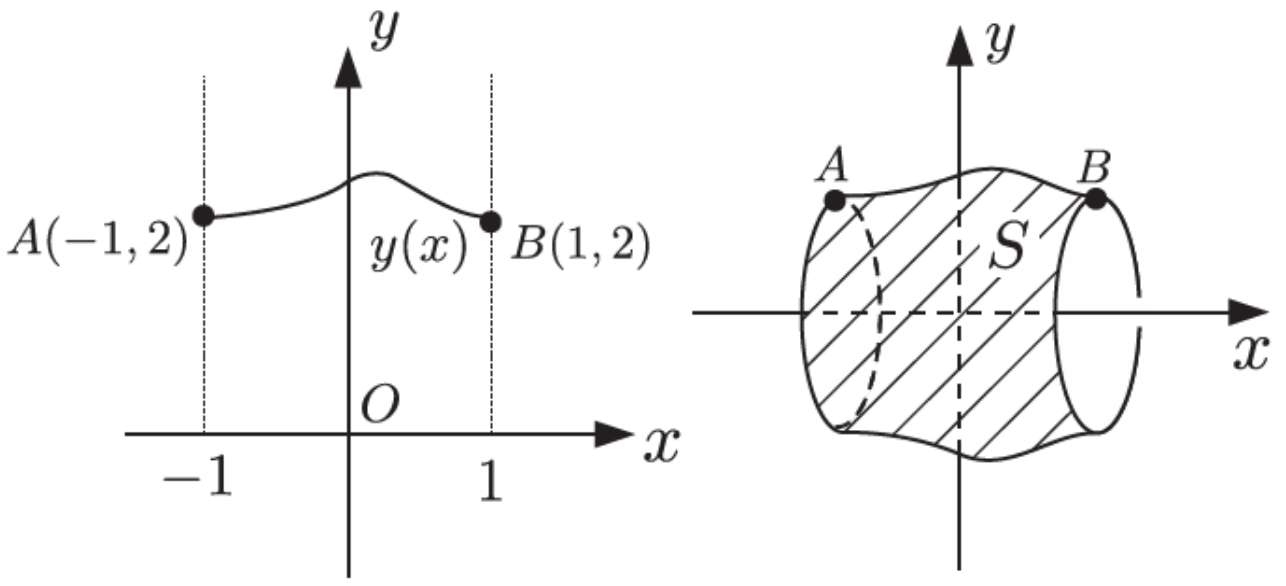
\includegraphics[width=11cm]{figure_2016_01.png}
\end{screen}

\begin{screen}
 (1) 表面積$S$が以下の式で表されることを示せ.
 \begin{align*}
  S &= 2 \pi \int_{-1}^1 F(y,y') \mathrm{d}x,\tag{2.1} \\
  F(y,y') &=y \sqrt{ 1 + \left(y'\right)^2}. \tag{2.2}
 \end{align*}
 ただし$\ds y' = \diff{}{y}{x}$である.
\end{screen}

$x$の増分が$\mathrm{d}x$のときの,表面積の増分$\mathrm{d}S$は,高さ$dx$,半径$y$および$y+y'\mathrm{d}x$の円錐台の側面積で近似できる.

\begin{align*}
 \mathrm{d}S &\approx \pi (2y+y'\mathrm{d}x) \sqrt{(\mathrm{d}x)^2+(y'\mathrm{d}x)^2} \\
 &\approx 2 \pi y \sqrt{1+(y')}\mathrm{d}x \\
 \therefore S &= \int_{-1}^{1} 2 \pi y \sqrt{1+(y')}\mathrm{d}x \\
 &= 2 \pi \int_{-1}^1 F(y,y') \mathrm{d}x
\end{align*}

\begin{screen}
 (2) 曲線$y(x)$は任意の$x$に対して以下のオイラー・ラグランジュ方程式を満たすとする.
 \begin{align*}
  \pdiff{}{F}{y} - \diff{}{}{x}\pdiff{}{F}{y'} = 0. \tag{2.3}
 \end{align*}
 $\ds \diff{}{F}{x}$と式(2.3)を考えることで,以下の関係式が成り立つことを示せ.
 \begin{align*}
  F - y'\pdiff{}{F}{y'} = c. \tag{2.4}
 \end{align*}
 ただし$c$はある定数である.
\end{screen}

\begin{align*}
 \diff{}{}{x}\left(F - y'\pdiff{}{F}{y'}\right) &= \left(y' \pdiff{}{F}{y} + y'' \pdiff{}{F}{y'}\right) - \left(y''\pdiff{}{F}{y'} - y' \diff{}{}{x} \pdiff{}{F}{y'}\right) \\
 &= y' \left(\pdiff{}{F}{y} - \diff{}{}{x}\pdiff{}{F}{y'}\right) \\
 &= 0
\end{align*}

よって,両辺を$x$で積分して$\ds F - y'\pdiff{}{F}{y'} = c$を得る.

\begin{screen}
 (3) 曲線 $y(x)$ が満たすべき微分方程式を$y,y',c$を用いて表わせ.
\end{screen}

$\ds \pdiff{}{F}{y'}= \frac{yy'}{\sqrt{1+\left(y'\right)^2}}$を代入して整理すると,
$$y=c\sqrt{1+\left(y'\right)^2}$$

\begin{screen}
 (4) 曲線 $y(x)$ を $x$ と $c$ を用いて表わせ.また,定数 $c$ が満たすべき方程式を求めよ.
\end{screen}

\begin{align*}
 &\diff{}{y}{x} = \pm \frac{\sqrt{y^2-c^2}}{c} \\
 &\Rightarrow \int \pm \frac{c}{\sqrt{y^2-c^2}} \mathrm{d}y = \int \mathrm{d}x
 \intertext{$y=c \cosh(t)$と置換する.$\mathrm{d}y = c \sinh(t)\mathrm{d}t$を用いて,} 
 &\Rightarrow \int \pm \frac{c}{\sqrt{c^2 \sinh^2 (t)}}\cdot c \sinh(t)\mathrm{d}t = x + D \\
 &\Rightarrow \int \pm |c| \mathrm{d}t = x + D \\
 &\Rightarrow t = \pm \frac{x+D}{|c|}
\end{align*}

以上により,$\ds y(x) = c \cosh \left(\pm \frac{x+D}{|c|}\right) = c \cosh \left( \frac{x+D}{c}\right) $となる.$y(-1)=y(1)=2$より,
$\ds c \cosh \left(\frac{-1+D}{c}\right) = c \cosh \left(\frac{1+D}{c}\right)=2$を満たす.$\cosh$のグラフの形から$D=0$が分かる.よって,$c$が満たすべき式は$\ds c \cosh\left(\frac{1}{c}\right) = 2$

\section{}

\begin{screen}
 以下の設問に答えよ.
\end{screen}

\begin{screen}
 (1) $n$ 個の同等な玉を,互いに区別できる $r$ 個の箱に入れる方法は何通りあるか.ただし,$n \geq 1, $ $1 \leq r \leq n$とし,どの箱にも少なくとも1個の玉が入るものとする.
\end{screen}

\begin{screen}
 次に,黒玉$n$個と白玉$m$個を無作為に1列に並べることを考える.同じ色のひと続きの並びを連と呼び,黒玉の連の個数を$r$,白玉の連の個数を$s$とする.ただし,$n \geq 1$ , $m \geq 1$ , $1 \leq r \leq n$ , $1  \leq s \leq m$とする.たとえば
 $$\underline{\mbox{●\hspace{1mm}●}}\hspace{1mm}\underline{\mbox{○\hspace{1mm}○\hspace{1mm}○}}\hspace{1mm}\underline{\mbox{●\hspace{1mm}●\hspace{1mm}●}}\hspace{1mm}\underline{\mbox{○\hspace{1mm}○}}\hspace{1mm}\underline{\mbox{●}}$$
 の場合は $r=3,s=2$となる.
\end{screen}

\begin{screen}
 (2) 黒玉同士,白玉同士を区別しないで並べる方法は全部で何通りなるか.
\end{screen}

\begin{screen}
 (3) 黒玉の連の個数が$r$,白玉の連の個数が$s$となる確率$P(r,s)$を求めよ.
\end{screen}

\begin{screen}
 (4) 黒玉の連の個数が$r$となる確率$P(r)$を求めよ.
\end{screen}

\begin{screen}
 (5) $(1+x)^n(1+x)^m = (1+x)^{n+m}$ を使って,次式が成り立つことを示せ.
 \begin{align*}
  \sum_{l=0}^{\min\{n,m\}}\binom{n}{l}\binom{m}{l} &= \binom{n+m}{m} \tag{3.1} \\
  \sum_{l=0}^{\min\{n-1,m\}} \binom{n}{l+1}\binom{m}{l} &= \binom{n+m}{m+1} \tag{3.2}
 \end{align*}
\end{screen}

\begin{screen}
 (6) $r$の期待値 $E(r)$ と分散 $V(r)$ を求めよ.また,$N=n+m,$ $\ds \lim_{N \rightarrow \infty}\frac{n}{N} = \lambda$とするとき \\ ($\lambda$は実数の定数),$\ds \lim_{N \rightarrow \infty}\frac{E(r)}{N}$と$\ds \lim_{N \rightarrow \infty}\frac{V(r)}{N}$を求めよ.

\end{screen}

\end{document}
